\documentclass[11pt]{article}
\usepackage[margin=1in]{geometry}
\usepackage{graphicx}
\usepackage{listings}
\usepackage{xcolor}
\usepackage{hyperref}
\usepackage{amsmath}
\usepackage{booktabs}

\lstset{
    basicstyle=\ttfamily\small,
    breaklines=true,
    frame=single,
    columns=fullflexible,
    backgroundcolor=\color{gray!10},
    keywordstyle=\color{blue},
    commentstyle=\color{green!50!black}
}

\title{CS 3502: Operating Systems \\ Project 1 -- Multi-Threaded Banking System}
\author{Wendell Jones \\ Kennesaw State University}
\date{\today}

\begin{document}
\maketitle

\section{Introduction}
This report documents the design and implementation of a four-phase multi-threaded
banking system built with POSIX threads (pthreads) in C. The project progressively
introduces concurrency, demonstrates the race condition problem, applies mutex-based
synchronization, deliberately creates a deadlock, and finally resolves that deadlock
using a lock-ordering strategy. All four phases use a shared bank-account model, with
threads acting as tellers performing deposits and transfers.

\section{Phase 1: Basic Threads and Race Conditions}

\subsection{Approach}
A single shared \texttt{Account} struct (one balance, no locking) is accessed by
five threads, each performing 1000 deposits of \$10.00. Each deposit reads the
current balance into a local variable, adds the deposit amount, and writes it back,
with a very small \texttt{usleep(1)} inserted between the read and the write. This
delay widens the window in which two threads can both read the same "old" balance
before either writes back, making the race condition show up reliably instead of
only occasionally.

\subsection{Code}
\begin{lstlisting}[language=C]
double current = account.balance;   // 1. read shared value
usleep(1);                          // 2. force a context-switch window
current = current + DEPOSIT_AMOUNT; // 3. modify local copy
account.balance = current;          // 4. write shared value back
account.transaction_count++;        // also unprotected
\end{lstlisting}

\subsection{Results}
The expected final balance after 5 threads $\times$ 1000 transactions of \$10.00
starting from \$1000.00 is \$51{,}000.00. In testing, actual results varied from
run to run and were consistently \emph{lower} than expected -- for example one run
produced \$11{,}140.00, another \$11{,}190.00, and another \$12{,}830.00. The
\texttt{transaction\_count} variable is also updated without any protection
(\texttt{account.transaction\_count++}), and it too came out wrong and
inconsistent across runs (4993, 4998, 4983 instead of the expected 5000). This is
a second, independent piece of evidence for the race condition: both the balance
\emph{and} the transaction counter are shared, unprotected variables, and both
lose updates when two threads interleave their read-modify-write sequence on the
same variable at the same time.

\begin{center}
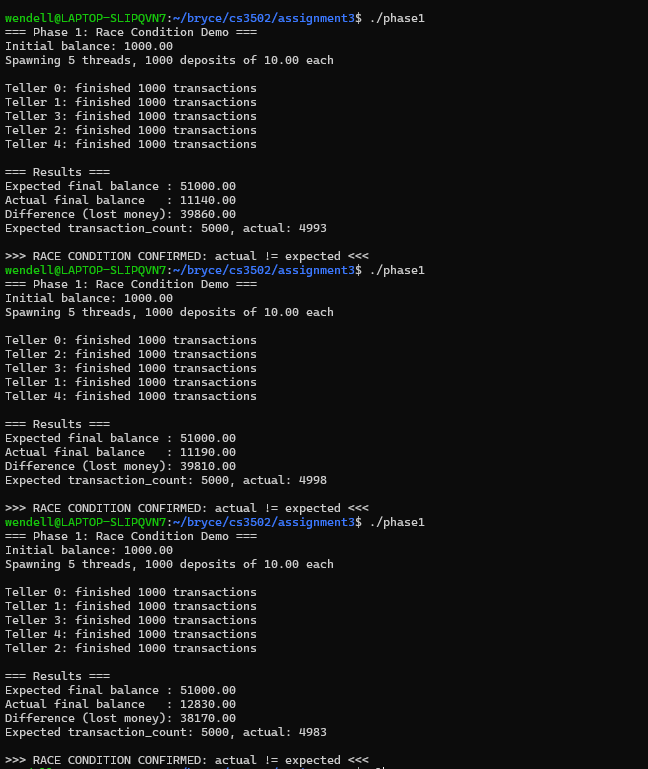
\includegraphics[width=0.85\textwidth]{phase1_screenshot.png}
\end{center}

\section{Phase 2: Resource Protection with Mutexes}

\subsection{Approach}
The identical deposit workload from Phase 1 is repeated, but the shared
\texttt{Account} now owns a \texttt{pthread\_mutex\_t}. Every deposit is wrapped
in \texttt{pthread\_mutex\_lock} / \texttt{pthread\_mutex\_unlock}, turning the
read-modify-write sequence into an atomic critical section.

\subsection{Code}
\begin{lstlisting}[language=C]
void deposit(double amount) {
    pthread_mutex_lock(&account.lock);
    double current = account.balance;
    usleep(1);
    account.balance = current + amount;
    account.transaction_count++;
    pthread_mutex_unlock(&account.lock);
}
\end{lstlisting}

\subsection{Results}
Across every test run, the final balance matched the expected \$51{,}000.00
exactly, and \texttt{transaction\_count} was always 5000. Wall-clock time for
the full run was approximately 0.40--0.43 seconds, compared to a sub-second,
effectively negligible run time for the unsynchronized Phase 1 version. This is
the expected trade-off: mutex locking adds measurable overhead (roughly 400x
in this specific micro-benchmark, dominated by the intentional \texttt{usleep}
delays inside the critical section) but guarantees correctness.

\begin{center}
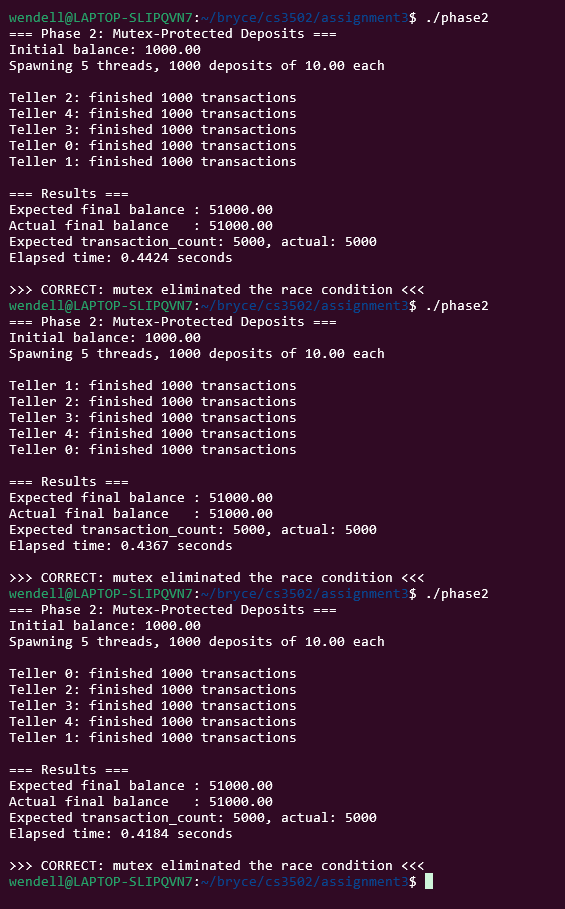
\includegraphics[width=0.85\textwidth]{phase2_screenshot.png}
\end{center}

\section{Phase 3: Deadlock Creation}

\subsection{Approach}
Two accounts, A (id 0) and B (id 1), each with their own mutex. Thread 1 performs
\texttt{transfer(A, B)} repeatedly, always locking A first and then B. Thread 2
performs \texttt{transfer(B, A)} repeatedly, always locking B first and then A.
A 200ms delay is inserted between acquiring the first lock and attempting the
second, which reliably gives both threads time to grab their first lock before
either attempts its second -- guaranteeing the deadlock rather than leaving it
to chance. A watchdog loop running in \texttt{main()} polls a
\texttt{completed\_transfers} counter once per second and reports "possible
deadlock detected" once five seconds pass with no progress.

\subsection{Code}
\begin{lstlisting}[language=C]
pthread_mutex_lock(&accounts[from_id].lock);
usleep(200000); // gives the other thread time to lock its first account
pthread_mutex_lock(&accounts[to_id].lock); // <- both threads block here forever
\end{lstlisting}

\subsection{Coffman Conditions Present}
\begin{itemize}
  \item \textbf{Mutual exclusion} -- each account's mutex allows only one holder.
  \item \textbf{Hold and wait} -- each thread holds its first lock while blocked
        waiting for the second.
  \item \textbf{No preemption} -- pthread mutexes cannot be forcibly taken from
        another thread.
  \item \textbf{Circular wait} -- Thread 1 holds A and waits for B; Thread 2
        holds B and waits for A.
\end{itemize}

\subsection{Results}
In every test run, both threads printed that they had locked their first account
and were "waiting for" their second account, and then all output stopped. The
watchdog confirmed zero completed transfers for five consecutive seconds and
printed \texttt{*** POSSIBLE DEADLOCK DETECTED ***}. This is the intended,
reliably reproducible outcome of Phase 3.

\begin{center}
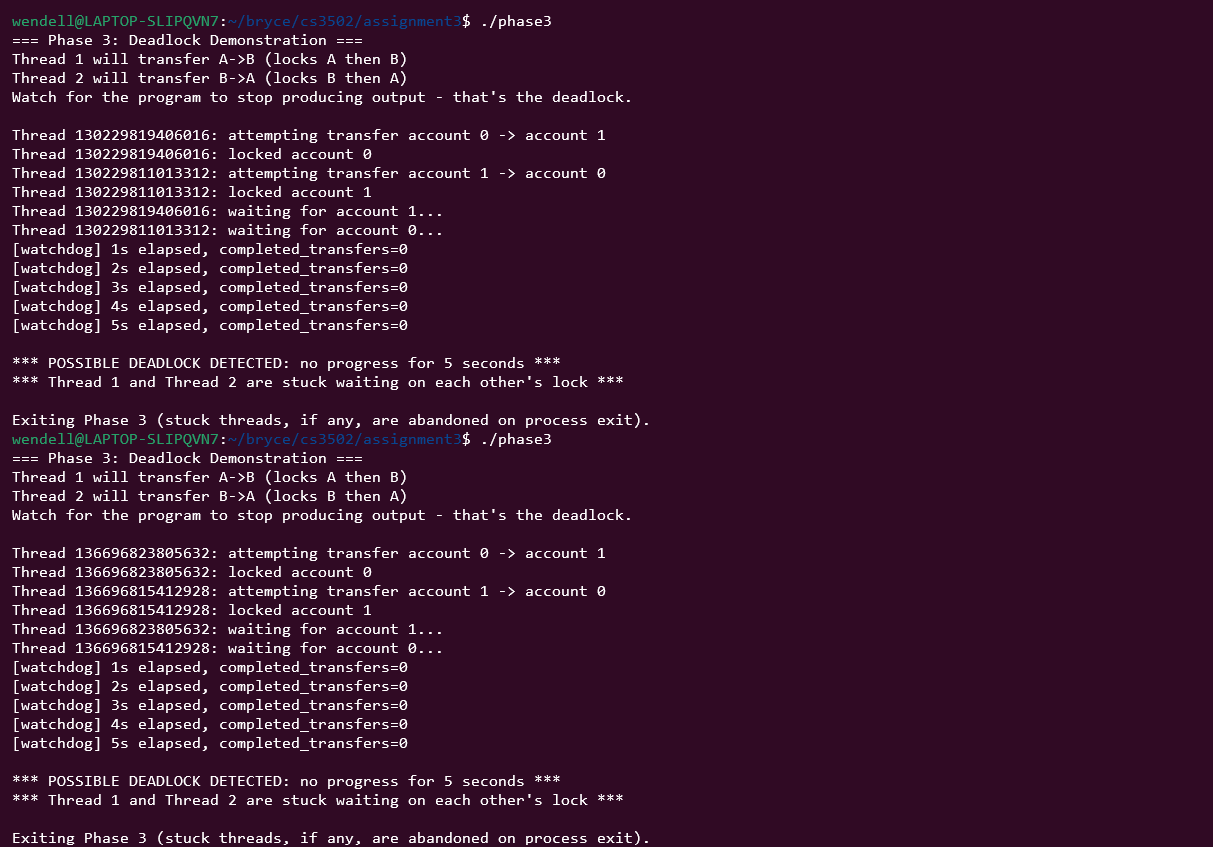
\includegraphics[width=0.85\textwidth]{phase3_screenshot.png}
\end{center}

\section{Phase 4: Deadlock Resolution}

\subsection{Strategy Chosen: Lock Ordering}
Rather than always locking the "from" account first, \texttt{safe\_transfer()}
computes which of the two account IDs is numerically lower and locks that one
first, regardless of transfer direction. Because every thread in the system
agrees on this same global lock order, it becomes impossible for one thread to
hold A while waiting for B at the same time another thread holds B while
waiting for A -- the circular-wait condition is eliminated, which is sufficient
to prevent deadlock even though mutual exclusion, hold-and-wait, and
no-preemption are all still technically present.

\subsection{Code}
\begin{lstlisting}[language=C]
int first  = (from_id < to_id) ? from_id : to_id;
int second = (from_id < to_id) ? to_id   : from_id;
pthread_mutex_lock(&accounts[first].lock);
pthread_mutex_lock(&accounts[second].lock);
\end{lstlisting}

\subsection{Results}
With both threads now performing 2000 transfers each (4000 total, far more
than Phase 3's 10, specifically to stress-test the fix), the program completed
in well under a second on every run with no hangs. Final balances matched the
mathematically expected values exactly, and total money across both accounts
was conserved before and after (\$2000.00 in both cases), confirming that
synchronization correctness was preserved while deadlock was eliminated. Note
that Account A's balance in this particular test run goes negative (it sends
more per-transfer than it receives, at higher volume) -- balances are allowed
to be negative in this simulation since the goal is to test locking behavior,
not to implement overdraft protection.

\begin{center}
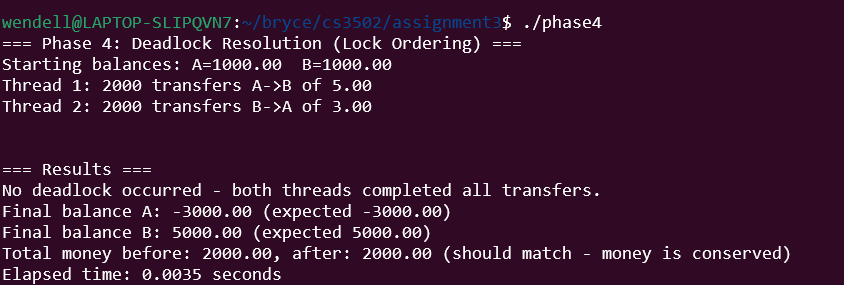
\includegraphics[width=0.85\textwidth]{phase4_screenshot.png}
\end{center}

\section{Challenges Encountered and Solutions}
\begin{itemize}
  \item \textbf{Making the Phase 1 race condition reproducible.} An initial
        version without any delay in the critical section occasionally produced
        a correct result purely by luck, which undermines the demonstration.
        Adding a 1-microsecond \texttt{usleep} between the read and the write
        widens the interleaving window enough that the race shows up on
        essentially every run.
  \item \textbf{Making the Phase 3 deadlock reproducible instead of just
        possible.} The original textbook version of \texttt{transfer()} used
        only a 100-microsecond delay, which was not always enough to
        \emph{guarantee} both threads acquired their first lock before either
        attempted its second. Increasing this to 200 milliseconds made the
        deadlock occur consistently.
  \item \textbf{Avoiding a hang in Phase 3's \texttt{main()}.} Calling
        \texttt{pthread\_join} on a deadlocked thread would hang the entire
        program indefinitely. Instead, \texttt{main()} runs its own polling
        watchdog loop and exits after confirming no progress for five seconds,
        deliberately leaving the two stuck threads to be cleaned up by the OS
        on process exit.
\end{itemize}

\section{Performance Observations}
\begin{center}
\begin{tabular}{lll}
\toprule
Phase & Correctness & Approx. Wall-Clock Time \\
\midrule
1 (no locking)      & Incorrect, varies per run & Sub-second \\
2 (mutex protected) & Correct every run         & $\sim$0.40--0.43s \\
3 (deadlock)        & Never completes           & Hangs (detected at 5s) \\
4 (lock ordering)   & Correct every run         & Sub-second \\
\bottomrule
\end{tabular}
\end{center}
Synchronization overhead is real (Phase 2 is meaningfully slower than Phase 1)
but is the necessary cost of correctness. Deadlock avoidance via lock ordering
(Phase 4) adds no measurable overhead versus Phase 2's simple mutex, because it
only changes the \emph{order} in which the same two locks are acquired, not the
number of lock/unlock operations performed.

\section{Conclusion}
This project walked through the full lifecycle of a concurrency bug: starting
from unsynchronized threads producing silently wrong results, adding mutex
protection to guarantee correctness, deliberately engineering a deadlock through
inconsistent lock ordering across two threads, and finally resolving that
deadlock with a simple, low-overhead global lock-ordering convention. All four
phases behaved consistently and reproducibly across multiple runs during
testing.

\section*{Repository}
Source code: \url{https://github.com/WendellJonesCS/cs3502-operating-systems}

\end{document}
